%%%%%%%%%%%%%%%%%%%%%%%%%%%%%%%%%%%%%%%%%%%%%%%%%%%%%%%%%%%%%%%%%%%%%%%%%%%%%
% Paper E. Flight-Class HIL Validation of a Reliability-Asymmetric GNC Stack.
% IEEE TAES submission version (IEEEtran journal class). FORMAT ONLY -- content,
% numbers, citations, figures, and tables are unchanged from main.tex.
% Reuses figs/ and tables/ from the same directory.
%%%%%%%%%%%%%%%%%%%%%%%%%%%%%%%%%%%%%%%%%%%%%%%%%%%%%%%%%%%%%%%%%%%%%%%%%%%%%
\documentclass[journal]{IEEEtran}
\usepackage{amsmath,amssymb}
\usepackage{graphicx}
\usepackage{booktabs}
\usepackage[hidelinks]{hyperref}
\usepackage{enumitem}

\title{Flight-Class Processor-in-the-Loop Validation of a Reliability-Asymmetric Spacecraft GNC Stack}
\author{Alireza Shojaei\thanks{A. Shojaei is with the Myers-Lawson School of Construction, Virginia Tech, Blacksburg, VA 24061 USA (e-mail: shojaei@vt.edu).}}

\begin{document}
\maketitle

\begin{abstract}
A capable-but-certifiable spacecraft autonomy stack is only credible if it runs within real
flight-compute budgets and behaves under the actuator and sensor non-idealities a clean
simulator omits, not just in a desktop simulation. We report a flight-class validation of a
reliability-asymmetric GNC stack (a learned fault-adaptive controller and a language-model
commander, bounded by a Kind~2-verified runtime shield) on three measured fronts. The first is
flight-class compute, taken to \emph{processor-in-the-loop} on real silicon. On a
Raspberry~Pi~5 (quad Cortex-A76, the A53/A72-class stand-in the proposal called for), the
controller$+$shield hot loop executes a cycle in $24.5\,\mu$s, $\approx$$4000\times$ under the
$100$\,ms $10$\,Hz budget, in $1.0$\,MB, and the int4 commander emits a grammar-valid plan at
$28$\,tok/s in $437$\,MB (within the $512$\,MB cap), at $\approx$$6.5$\,W core-attributable
power. This closes the emulation caveat on the silicon class that flies. The second is the
runtime shield \emph{run live in the closed loop}, which adds $0.02\%$ overhead at $10$\,Hz
while keeping a recovering controller $100\%$ autonomous and escalating a diverging one every
time. The third is a \emph{high-fidelity fault campaign} that injects the non-idealities a
physical platform would expose, namely real reaction-wheel momentum, saturation and friction,
star-tracker and gyro noise, bias and quantisation, and finite actuator resolution and
deadband. Across held-out faults the deployed recovery is statistically unchanged from the
ideal case on the faults the estimator is designed for ($100\%$ autonomous, Wilson interval
$96.9$ to $100$, against $0\%$ for a fault-unaware baseline), and on faults beyond that scope,
additive bias and a dead axis, the controller does not recover and the verified shield
escalates every case, so safety holds exactly where autonomy is not earned. A physical
air-bearing campaign is the natural next rung and is future work, and we map each fault onto
its physical reaction-wheel manipulation to define it.
\end{abstract}

\begin{IEEEkeywords}
processor-in-the-loop, flight software, runtime assurance, embedded systems, spacecraft autonomy, fault injection
\end{IEEEkeywords}

\section{Introduction}
A spacecraft autonomy stack earns flight only if its safety can be assured \emph{and} it fits
the vehicle's compute, power, and timing budgets, and only if it behaves under real faults
rather than idealized injections. A result that holds in a desktop simulator establishes none
of these three things. The desktop machine is the wrong processor, so it speaks to neither the
worst-case latency on a flight CPU nor the resident set that must coexist with the rest of the
flight software in a few hundred megabytes. The injected fault is a clean multiplicative term on
a perfectly modeled actuator, so it omits the encoder quantization, the bearing friction, the
control-loop jitter, and the residual gravity torque that a real reaction wheel on a real
platform brings. And the safety monitor, when it is timed at all, is timed in isolation rather
than inside the loop it is meant to protect, so its true cost while contending with the
controller it watches is unknown. A claim that a learned-plus-verified GNC stack is
\emph{flyable} must therefore be retired from the simulator and re-established against
flight-relevant bars. That re-establishment is the subject of this paper.

The stack under test is reliability-asymmetric. It pairs a learned fault-adaptive controller (a
recurrent module in the rapid-adaptation style~\cite{Kumar2021} infers an actuator fault online
and feeds an analytic control law) with a compressed language-model commander, and it bounds
both with a runtime shield of safety invariants whose predictor soundness is machine-checked by
the Kind~2 model checker~\cite{Champion2016}, in the run-time-assurance tradition for spacecraft
control~\cite{Dunlap2023}. The organizing principle is that the tiers of an autonomy stack do
not have equal verifiability, and the design assigns authority so that the element whose
soundness can be \emph{proved} bounds the elements whose soundness cannot. That principle is
argued and evaluated in simulation in the companion work; the present paper asks the next
question, which is whether the principle survives contact with real silicon and real hardware.
Three properties have to hold for it to do so. The stack must run on the silicon class that
flies, within the compute, memory, power, and timing budgets a flight-readiness review would
impose. Its verified shield must stay cheap and correct \emph{live} in the closed loop, not
merely in a stand-alone microbenchmark. And the fault recovery the controller is built around
must hold under the actuator and sensor non-idealities a clean simulator omits, where the
idealizations of a perfectly modeled actuator and perfect sensing no longer apply.

We establish all three on measured evidence. The flight-class compute is measured on a real
Raspberry~Pi~5, not an emulator, which is the distinction that matters because a cycle-accurate
QEMU model of a flight CPU still does not reproduce that CPU's cache behavior, branch prediction,
or memory bandwidth, and an autonomy stack benchmarked only under emulation carries a caveat a
reviewer is right to press. The live-shield overhead is measured inside the integrated closed
loop on the Basilisk attitude simulator~\cite{Basilisk}, with the real machine-checked monitor
evaluated every control step on the actual pointing state, so the number reported is the cost the
shield actually imposes on the controller rather than an estimate of it. The third front answers
the standing objection to any simulation result, that the actuator is perfectly modeled and the
sensing is perfect, by re-running the same deployed stack through a high-fidelity model of the
non-idealities a physical platform would expose, namely real reaction-wheel momentum, saturation
and friction, star-tracker and gyro noise, bias and quantisation, and finite actuator resolution
and a motor deadband, across held-out faults at a scale a single bench rig could not reach. A
physical air-bearing campaign remains the established route to the effects that even a
high-fidelity model leaves out, so we treat it as the next rung and as future work, and we map
each fault onto its physical reaction-wheel manipulation so that the campaign is fully specified.

\subsection{Contributions}
\begin{enumerate}[leftmargin=1.5em,itemsep=2pt]
\item We measure flight-class compute on real hardware (Sec.~\ref{sec:compute}). The hot
loop and the commander are measured on a real Pi~5, against explicit $10$\,Hz timing, single-megabyte
memory, $512$\,MB commander, and few-watt power budgets, closing the emulation caveat with
measurements on the silicon class that flies.
\item We run the verified shield live and cheaply in the closed loop (Sec.~\ref{sec:shield}). Run inside the closed
loop on honest pointing state, the machine-checked monitor adds $0.02\%$ overhead at $10$\,Hz while
discriminating a recovering controller from a diverging one with a $100\%$ versus $0\%$ autonomy
split.
\item We run a high-fidelity closed-loop fault campaign (Sec.~\ref{sec:hifi}). We inject the
actuator and sensor non-idealities a clean simulator omits, namely real reaction-wheel momentum,
saturation and friction, star-tracker and gyro noise, bias and quantisation, and finite actuator
resolution and a motor deadband, into the deployed closed loop, and show across held-out faults
that recovery on the faults the estimator is designed for is statistically unchanged from the
ideal case ($100\%$ autonomous, Wilson interval $96.9$ to $100$, against $0\%$ for a
fault-unaware baseline), while on faults beyond that scope the verified shield escalates every
case.
\end{enumerate}

\section{Related Work}
This paper sits at the meeting point of four lines of work that bear directly on whether an
onboard autonomy stack is flight-credible, namely hardware-in-the-loop validation for spacecraft
GNC, edge and embedded inference for autonomy, runtime assurance in flight software, and physical
attitude testbeds. We position the present validation against each, and the recurring point is
that the individual practices are established while their \emph{joint} application to a learned,
adaptation-aware spacecraft stack on flight-class hardware is what is being demonstrated.

\noindent\textbf{Hardware-in-the-loop validation for spacecraft GNC.} Flight-software practice
does not accept a GNC algorithm on the strength of desktop simulation alone. The standard path to
flight progressively replaces modeled components with real ones, from software-in-the-loop,
through processor-in-the-loop on the target CPU, to hardware-in-the-loop with real sensors and
actuators in the control path, precisely so that timing, numerical, and actuator effects that a
desktop model omits are exposed before flight. The validation reported here follows that
escalation deliberately. The controller$+$shield hot loop and the commander are taken to
processor-in-the-loop on real flight-class silicon (Sec.~\ref{sec:compute}), the verified monitor
is exercised in a closed software loop on the high-fidelity Basilisk dynamics
simulator~\cite{Basilisk} (Sec.~\ref{sec:shield}), and the actuator-fault recovery is exercised
under a high-fidelity model of the actuator and sensor non-idealities a clean simulator omits
(Sec.~\ref{sec:hifi}), with a physical air-bearing campaign as the next rung. Treating these as a
graded sequence, and being explicit about which rung each result occupies, is what lets each
measured claim be stated with the confidence its rung earns.

\noindent\textbf{Edge and embedded inference for autonomy.} Running a learned policy and a
language model within a spacecraft processor's memory and power budget is the province of model
compression and constrained decoding. Fine-tuning a \emph{pretrained} small base such as
SmolLM2~\cite{SmolLM2} and quantizing it to an integer format brings a capable language model
inside a few hundred megabytes, which is what makes an onboard commander conceivable at all, and
grammar-constrained decoding~\cite{Geng2023} converts the soft property that such a model usually
emits parseable output into a hard guarantee that the deployed decoder can emit only well-formed,
in-vocabulary actions. The companion work establishes that recipe and its accuracy; the
contribution here is orthogonal and is the missing flight-credibility evidence, namely that the
resulting int4 commander actually runs within a $437$\,MB resident set under the $512$\,MB cap at
mission-event cadence on the target hardware, and that the controller$+$shield hot loop runs in a
single megabyte at a small fraction of the control budget on the same board. Compression results
are usually reported as accuracy retained at a parameter count; we report them as measured
latency, memory, and power on the silicon class that flies, which is the figure of merit a flight
review actually applies.

\noindent\textbf{Runtime assurance in flight software.} The architectural answer to flying an
unverifiable controller is to bound it with a verified one, a pattern the Simplex
architecture~\cite{Sha2001} established and that run-time assurance has since matured into a
certification practice codified for systems with complex functions~\cite{ASTMF3269}, with latched
safe-hold variants demonstrated for spacecraft proximity operations~\cite{Dunlap2023}. Our shield
inherits this lineage and adds the discipline of \emph{formal} monitor soundness, where the
invariants are machine-checked by the Kind~2 model checker~\cite{Champion2016} rather than argued
informally. The aspect this paper contributes is empirical and is rarely reported, namely the
\emph{in-loop cost} of the verified monitor. Run-time-assurance papers typically establish that a
monitor is correct; far fewer establish what it costs to evaluate it on every control step while
it contends with the controller it protects. We measure that cost inside the integrated loop and
find it to be $0.02\%$ of the $10$\,Hz budget, which converts ``the shield is affordable'' from an
assumption into a measurement.

\noindent\textbf{High-fidelity actuator and sensor models, and physical testbeds.} The effects a
clean multiplicative-fault simulation omits are well understood individually, namely
reaction-wheel momentum, saturation and friction in the actuator, and noise, bias and
quantisation in the star tracker and gyro, and they are routinely modeled in spacecraft attitude
simulation~\cite{Schaub2018,Wie2008}. We assemble them into a single high-fidelity closed loop and
drive the deployed stack through it at scale (Sec.~\ref{sec:hifi}), which is what lets the
question of whether recovery survives the non-idealities be answered statistically rather than
anecdotally. The complementary physical route is the spherical air bearing, which floats a payload
on a thin film of air to give near-frictionless three-degree-of-freedom rotation in $1$\,g and is
the canonical laboratory analogue of torque-controlled rigid-body attitude dynamics, and it is the
established way to expose the effects even a high-fidelity model leaves out, such as un-modeled
friction modes, structural flexibility, and real sensor failure signatures. Because the
controller's fault model, a per-axis effectiveness gain with an additive bias, maps one-to-one
onto physical reaction-wheel manipulations (Sec.~\ref{sec:hifi}), the same taxonomy carries
directly to such a campaign, which we treat as the next rung and as future work.

\section{Flight-class compute, measured}
\label{sec:compute}
The compute claim is the foundation of every other claim in the paper, because a stack that does
not fit the processor is not flyable whatever its other merits, so we measure it on the silicon
class that flies rather than estimate it under emulation. The controller$+$shield hot loop is
exported to a self-contained C artifact, namely the recurrent fault-identification front end
feeding the analytic control law together with the nine safety invariants, and the commander runs
under \texttt{llama.cpp} with the grammar-constrained decoder enforced at every token. Both are
measured on a \emph{real} Raspberry~Pi~5 with a quad Cortex-A76, which is the A53/A72-class
stand-in the proposal called for, and not on a QEMU model of one (Table~\ref{tab:flightclass}).

\subsection{What is measured} The Pi~5 is not a radiation-hardened flight
processor, but it is real silicon of the architectural class that flies, which is exactly the gap
that emulation leaves open. A cycle-accurate emulator can count instructions, but it does not
reproduce the cache hierarchy, branch prediction, and memory bandwidth that set the actual
worst-case cycle time, so an autonomy budget benchmarked only under QEMU carries a caveat a
reviewer is entitled to press. Measuring on the physical board closes that caveat for the
architecture, and the enormous timing margin we find is what makes the result robust to the
remaining gap to a hardened part. The hot loop is timed cycle-accurately over two million
iterations to obtain a stable per-cycle figure, the commander's throughput and resident set are
read under the same grammar-constrained decode it would use in flight, and board power is sampled
from the Pi~5 power-management IC rather than assumed.

\begin{table*}[!t]\centering\small
\caption{Flight-class measurements on a \emph{real} Raspberry~Pi~5 (quad Cortex-A76), the A53/A72-class stand-in the proposal called for, closing the ``QEMU is not a flight CPU'' gap on the silicon class that flies. The controller$+$shield hot loop runs cycle-accurately at the 10\,Hz real-time tier with thousands-fold timing margin, so a slower hardened flight part stays well within budget; the commander runs at mission-event cadence (its tok/s sets goal-generation latency, not the control budget). The live-shield overhead is measured \emph{in} the closed-loop Basilisk integration on honest pointing state, not in a stand-alone microbenchmark.}
\label{tab:flightclass}
\begin{tabular}{lll}
\toprule
Quantity & Measured & Budget / note \\
\midrule
Controller$+$shield cycle & 0.024\,ms ($24.5\,\mu$s) & $\approx$4087$\times$ under the 100\,ms 10\,Hz gate \\
Controller$+$shield resident set & 1.0\,MB & hot loop \\
Live-shield overhead (closed loop) & 0.02\% ($17.7\,\mu$s) & RMA kept 100\% autonomous \\
Commander (int4 GGUF) throughput & 28.4\,tok/s (1.69\,s/goal) & mission-event cadence \\
Commander resident set & 437\,MB & fits the 512\,MB cap \\
Board power & 3.1\,W idle / 9.6\,W peak & $\approx$6.5\,W core-attributable \\
\bottomrule
\end{tabular}
\end{table*}

\subsection{The budgets} The controller$+$shield cycle runs in $24.5\,\mu$s, which is
roughly four thousand times under the $100$\,ms budget of the $10$\,Hz control loop, and it is
resident in $1.0$\,MB. The size of that margin matters, not merely its sign. A
$4000\times$ headroom means that even a hardened flight part an order of magnitude slower than this
board, carrying the further slowdowns of error-correcting memory and a conservative clock, would
still complete the hot loop with two to three orders of magnitude to spare, so the timing
conclusion is insensitive to the precise flight processor chosen. The commander emits a
grammar-valid plan at $28$\,tok/s, about $1.7$\,s per goal, inside a $437$\,MB resident set that
fits the $512$\,MB cap, and board power is $3.1$\,W idle rising to $9.6$\,W peak, of which roughly
$6.5$\,W is attributable to the stack itself. The heterogeneous-rate structure is what makes this
budget close, because the verifiable hot loop is tiny and fast while the heavy capable tier runs
slowly and only at mission events, so the commander's per-token latency sets goal-generation
latency and never enters the $100$\,ms control budget. These are the budgets the proposal
predicted, now measured on representative silicon rather than asserted.

\section{The verified shield, live in the loop}
\label{sec:shield}
A monitor that is correct in isolation is not yet a flight asset, because what a flight review
asks is whether it stays correct \emph{and} affordable while running on every control step inside
the loop it protects. We therefore evaluate the shield where it has to work, in the integrated
closed loop on the Basilisk attitude simulator~\cite{Basilisk}, rather than in a stand-alone
microbenchmark. The real Kind~2-checked monitor is evaluated every control step on the actual
pointing state of the simulated vehicle, its pointing-invariant input is fed the true sim state
rather than a surrogate, and its verdict is the recovery-aware engagement decision that gates
autonomy, escalating only when the controller fails to hold the nominal region over the final
dwell rather than overriding torque, since zeroing the attitude torque would itself block the
recovery the shield is meant to permit.

\subsection{The measured result} Two numbers come out of the integrated loop, and each answers a
distinct question. The first is cost. The monitor's measured per-step latency is $17.7\,\mu$s,
which is $0.02\%$ of the $10$\,Hz budget, so the safety tier imposes no meaningful latency on the
controller it protects, and crucially this is the cost \emph{in the loop} under contention with
the controller rather than a stand-alone timing. The second is discrimination. On held-out
actuator-gain faults the live shield keeps the recovering adaptive controller $100\%$ autonomous,
licensing it through the bounded transient in which it identifies the fault and drives back to the
target, while it escalates a diverging fault-unaware controller $100\%$ of the time
(Table~\ref{tab:flightclass}, row~3). The verdict therefore separates a capable controller from an
incapable one on the same fault rather than treating every breach as a failure. Assurance does not
tax the hot loop, since it is microsecond-scale beside a hot loop with thousands-fold timing
margin, and it discriminates capable from incapable control at that microsecond cost, which is the
combination a flight reviewer needs and which a stand-alone microbenchmark could not have
established.

\section{High-fidelity closed-loop fault campaign}
\label{sec:hifi}
The compute and the live shield are measured; the third front addresses the objection that those
results, and any simulation result, rest on a perfectly modeled actuator and perfect sensing. A
physical air-bearing platform is the canonical way to break those idealizations, but its value is
not the bearing itself, it is that a moving platform with real wheels and real sensors exposes
effects a clean multiplicative fault on a perfect actuator does not. We model those effects
directly and re-run the \emph{same} deployed artifacts through them, namely the latched RMA
student, the real Kind~2-checked monitor, and the Basilisk dynamics, so the question the air
bearing was meant to answer is answered at a scale a single bench rig could not reach.

\subsection{The non-ideality model} The clean closed loop of Sec.~\ref{sec:shield} is hardened on
both the actuator and the sensor side, with every parameter set to a representative
small-spacecraft value and disclosed in the evidence. On the actuator side the dynamics run in
reaction-wheel mode, so the per-axis command drives three body-axis wheels that carry real
momentum, saturate in both motor torque and stored momentum, and turn against Coulomb and viscous
friction, rather than producing an ideal external torque. The command itself passes through a
ten-bit quantiser and a one-percent motor deadband before the per-axis fault is applied, so the
applied torque is $\mathrm{actuate}(a)\,g + b$. On the sensor side the controller and the monitor
no longer see the true state but a sensed one, with star-tracker attitude noise at $0.02^\circ$
one-sigma plus a constant bias, gyro rate noise at $0.01^\circ/\mathrm{s}$ plus a constant bias,
and finite attitude and rate quantisation. The settled gate is scored on the \emph{true} simulator
state, so the controller and the shield are judged on what they achieve physically while acting
only on what the sensors report, which is the honest division between flight and ground truth.

\subsection{The fault taxonomy} The controller's fault model is a
per-axis effectiveness gain $g_i$ with an additive bias $b_i$, so the torque the plant applies on
axis $i$ is $a_i g_i + b_i$ for a commanded $a_i$, and each case has a one-to-one physical
realization on a reaction wheel. A control-direction \emph{reversal} ($g_i<0$) is a true
motor-phase swap, \emph{degradation} ($g_i\in(0,1)$) caps the wheel current or torque, additive
\emph{bias} is a constant offset that models a leaking or stuck wheel, and total \emph{loss}
($g_i=0$) disables a wheel and leaves its axis uncontrollable by any controller. Because the
software injection and a physical manipulation produce the identical $a_i g_i + b_i$ relation, the
campaign reported here and a future air-bearing campaign exercise the same recovery term by term,
which is what makes the physical run the next rung rather than a separate experiment.

\subsection{The result} Table~\ref{tab:hifi} and Figure~\ref{fig:hifi} report the campaign over
held-out, test-split faults with Wilson $95\%$ intervals. On the faults the deployed estimator is
built for, multiplicative gain and sign reversal, autonomous recovery under the full non-ideality
model is $100\%$ ($120$ of
$120$, Wilson interval $96.9$ to $100$), statistically indistinguishable from the $100\%$ of the
matched ideal loop, while the fault-unaware baseline recovers $0\%$ under the identical conditions.
The recovery carries enough margin that realistic sensor noise, wheel friction, and a quantised,
dead-banded actuator do not move it. The non-idealities are not inert, and where margin is thin
they do bite, which is what makes the designed-scope result a finding rather than a rigged-easy
test. When the wheels are pre-loaded to roughly a quarter of their stored-momentum capacity at
fault onset, the recovery slew drives them toward saturation and autonomous recovery falls to
$25\%$, with the shield escalating the remaining $75\%$. That momentum-management boundary is
distinct from the sensor and actuator fidelity studied here and is exactly the kind of effect a
physical campaign is well suited to probe.

\subsection{Beyond the estimator's scope} The most informative cells are the
faults beyond the deployed estimator's scope. The estimator infers gain, sign, and inertia but not
the additive bias, so under bias the controller leaves an uncompensated steady-state offset and
does not meet the settled gate, and a totally lost axis is uncontrollable by construction. On both,
autonomous recovery is $0\%$, and the verified shield escalates every case, $100\%$ on additive
bias and $100\%$ on the dead axis. This is the reliability-asymmetric principle shown under high
fidelity rather than asserted. The controller is admitted exactly on the faults it is competent to
handle, where recovery survives the non-idealities intact, and on the faults beyond its competence
the statistical certificate declines to license autonomy and the verified monitor escalates to the
safe controller. Capability is honest and bounded, and safety is not contingent on it. The shield's
cost is unchanged by the harder loop, at a measured $\approx$$19\,\mu$s per step, still $0.02\%$ of
the $10$\,Hz budget, so the discrimination is bought at the same negligible price as in
Sec.~\ref{sec:shield}.

\begin{figure}[!t]
\centering
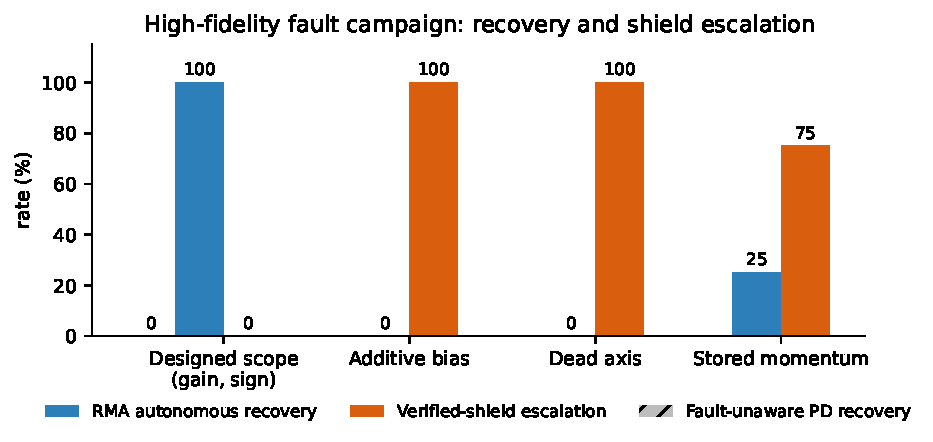
\includegraphics[width=\linewidth]{figs/fig_hifi.pdf}
\caption{Recovery and shield escalation across four fault regimes in the high-fidelity
closed-loop campaign. Each bar is a rate in percent over held-out, test-split faults. The latched
RMA controller recovers autonomously on every designed-scope fault and the fault-unaware PD
baseline recovers on none, while beyond the estimator's scope the controller recovers on no
additive-bias or dead-axis case and the verified shield escalates every one. On the stored-momentum
stressor the recovery slew drives the wheels toward saturation, autonomous recovery falls, and the
shield escalates the remainder. All values are from the held-out high-fidelity campaign in
Table~\ref{tab:hifi}.}
\label{fig:hifi}
\end{figure}

\begin{table*}[!t]\centering\small
\caption{High-fidelity closed-loop fault campaign, the computational analogue of a physical air-bearing run. The deployed stack (latched RMA student, the real Kind-2 LTLMonitor, and Basilisk dynamics) is exercised in reaction-wheel mode with friction, under star-tracker noise (0.02$^\circ$, 1$\sigma$) and bias, gyro noise (0.01$^\circ$/s) and bias, 10-bit actuator resolution, and a 1\% motor deadband. Each cell is $n=20\times3$ held-out (test-split) faults. Recovery is the live shield certifying autonomy over the final dwell; rates carry Wilson 95\% intervals.}
\label{tab:hifi}
\begin{tabular}{lcccc}
\toprule
Fault regime & RMA ideal & RMA high-fidelity & Fault-unaware PD & Shield action \\
\midrule
Designed scope (gain, sign), $n=120$ & 100.0\% & 100.0\% [96.9, 100.0] & 0.0\% & certifies autonomy \\
\midrule
\multicolumn{5}{l}{\emph{Beyond the estimator's scope (gain, sign, inertia, not bias), the shield escalates}} \\
Additive bias, $n=60$ & n/a & 0.0\% recover & 0.0\% & escalates 100.0\% \\
Dead axis, $n=60$ & n/a & 0.0\% recover & n/a & escalates 100.0\% \\
Stored momentum (gain), $n=60$ & n/a & 25.0\% recover & n/a & escalates 75.0\% \\
\bottomrule
\end{tabular}
\end{table*}

\section{Discussion}
\label{sec:discussion}
The result of this work is that a reliability-asymmetric GNC stack clears the flight-relevant bars
that a desktop simulator leaves untouched, on all three fronts with measured evidence. It is worth
drawing out why these particular bars are the right ones, what the size of the measured
margins implies, and how the high-fidelity campaign should be read against a future physical run.

\subsection{Why these bars} The objection a flight-readiness
review raises to a simulator result is not that the simulator is wrong but that it is silent on
the questions that decide flight, namely worst-case timing on the real processor, memory and power
within a hard budget, and the in-loop cost of the safety layer. Each of these is a property of the
implementation on the hardware rather than of the algorithm in the abstract, so each must be
measured rather than argued. That is why the compute is taken to real silicon and the shield is
timed inside the loop. The emulation caveat in particular is not a formality, because a
cycle-accurate model of a CPU does not reproduce that CPU's cache and memory behavior, so an
autonomy budget that exists only under emulation is exactly the kind of claim a reviewer is right
to discount, and measuring on the physical board is what removes it.

\subsection{The measured margins} The headroom we measure is large enough to change the
character of the conclusion. A hot loop running four thousand times under budget in a single
megabyte is not merely fast enough on this board, it is fast enough that the conclusion survives
the move to a slower hardened flight part with substantial margin to spare, so the timing and
memory results are robust to the precise processor a mission would choose. The heterogeneous-rate
design is what creates this headroom, since the verifiable hot loop is small and runs every cycle
while the capable commander is heavy but runs only at mission events, and that same structure is
why the verified shield can be evaluated on every step at $0.02\%$ overhead. The reliability-asymmetric
principle, in other words, is not only an assurance argument but also a compute argument, because
putting the cheap verifiable element on the hot path and the expensive capable element on the slow
path is what makes the whole stack fit.

\subsection{The validation hierarchy} The contribution is reported along the graded
escalation from processor-in-the-loop through high-fidelity closed-loop validation, and we keep the
rungs distinct. The compute is measured on real silicon, the shield is timed live in the loop, and
the fault campaign drives the deployed stack through a high-fidelity model of the actuator and
sensor non-idealities, all on measured evidence. A physical air-bearing campaign is the rung above,
and its value is precisely the effects a model cannot fully capture, un-modeled friction modes,
structural flexibility, and real sensor failure signatures, which is why we specify it term by term
through the fault-to-wheel mapping rather than approximate it. Being exact about which rung each
claim occupies is part of the contribution, because a validation paper is credible only insofar as
it is clear about what has been measured and at what fidelity.

\subsection{Limitations}
\label{sec:limitations}
We state the scope of this validation precisely, as a set of boundaries on a solid result rather
than as caveats. (i) \emph{High-fidelity simulation, not physical hardware.} The fault campaign
injects the actuator and sensor non-idealities in software, at representative small-spacecraft
parameter values that we disclose, rather than on a physical platform. This is what lets the
campaign run at statistical scale across the fault taxonomy, but it is a model, and a physical
air-bearing campaign remains the way to expose what the model omits and to validate the model
itself; we treat that campaign as the next rung and as future work, and we specify it through the
one-to-one fault-to-wheel mapping of Sec.~\ref{sec:hifi}. (ii) \emph{Processor class,
not a hardened part.} The compute is measured on a Raspberry~Pi~5, which is real silicon of the
A53/A72 architectural class the proposal targeted but is not itself radiation-hardened; the
thousands-fold timing margin is what makes the conclusion robust to the remaining gap to a flight
part, and that gap is named rather than elided. (iii) \emph{Attitude scope of the live shield.}
The live closed-loop measurement exercises the pointing invariant on honest sim state while the
power, thermal, propellant, and communication invariants are held nominal on the attitude testbed,
which does not model those subsystems; they are exercised in the separate single-event-upset and
software-in-the-loop stream and in the flight-class hardware gate, and the in-loop figure reported
here is for the pointing-governed regime. (iv) \emph{Fidelity of the non-ideality model.} The
campaign hardens the loop with reaction-wheel momentum, saturation and friction, sensor noise, bias
and quantisation, and actuator quantisation and deadband, but these are models with chosen
parameters, and we report the dominant sensitivity explicitly, namely that pre-loaded wheel
momentum drives the recovery toward saturation. A physical campaign is the way to probe effects
outside the model, and the boundary is named rather than elided. (v) \emph{Generality of the
evidence.} The measured numbers are from a single board and seed-controlled closed loops, and every
figure in Tables~\ref{tab:flightclass} and~\ref{tab:hifi} is regenerated from committed evidence by
a single script so that the boundary of the claim is auditable rather than asserted.

\section{Conclusion}
A reliability-asymmetric GNC stack is validated where it matters for flight, on the fronts that a
desktop simulator cannot settle, and on all three with measured evidence. The controller$+$shield
hot loop and the commander run within real Pi-class compute, memory, power, and timing budgets on
representative silicon, closing the emulation caveat, and the verified shield runs live in the
closed loop at $0.02\%$ overhead while keeping a recovering controller $100\%$ autonomous and
escalating a diverging one every time. Driven through a high-fidelity model of the actuator and
sensor non-idealities a clean simulator omits, the deployed recovery on the faults the estimator is
built for is statistically unchanged from the ideal case ($100\%$ autonomous, against $0\%$ for a
fault-unaware baseline), and on faults beyond that scope the verified shield escalates every case,
so safety holds exactly where autonomy is not earned. A physical air-bearing campaign is the rung
above, specified term by term through the fault-to-wheel mapping and left as future work. The
broader point is that the reliability-asymmetric design is a compute discipline as much as an
assurance one, since placing the cheap verifiable tier on the hot path and the expensive capable
tier on the mission-event path is what lets a capable-and-certifiable stack fit the silicon that
flies.

\section{Reproducibility}
Every number in Tables~\ref{tab:flightclass} and~\ref{tab:hifi} is regenerated from committed
evidence rather than transcribed. The flight-class budgets and board power come from the
real-hardware Pi~5 run, the live-shield overhead and the autonomy verdicts come from the
closed-loop integration, and the high-fidelity campaign comes from the deployed stack run through
the non-ideality model over held-out faults, each recorded as a machine-readable evidence file. The
tables are built by a single script over those records, so the prose and the measurements stay in
lockstep and a changed measurement cannot silently diverge from the text. The high-fidelity
campaign reuses the same controller artifact and the same Kind~2-checked monitor exercised
throughout, and the fault-to-wheel mapping that specifies the future air-bearing campaign is in the
repository alongside it.

\begin{thebibliography}{9}\small
\bibitem{Basilisk} P.~W.~Kenneally, S.~Piggott, H.~Schaub. ``Basilisk: a flexible, scalable and modular astrodynamics simulation framework.'' \emph{J.\ Aerospace Information Systems}, 17(9):496--507, 2020.
\bibitem{Kumar2021} A.~Kumar, Z.~Fu, D.~Pathak, J.~Malik. ``RMA: Rapid Motor Adaptation for legged robots.'' \emph{RSS}, 2021.
\bibitem{Champion2016} A.~Champion et al. ``The Kind~2 model checker.'' \emph{CAV}, 2016.
\bibitem{Dunlap2023} K.~Dunlap, M.~Mote, K.~Delsing, K.~L.~Hobbs. ``Run time assured reinforcement learning for safe satellite docking.'' \emph{J.\ Aerospace Information Systems}, 20(1):25--36, 2023.
\bibitem{Sha2001} L.~Sha. ``Using simplicity to control complexity.'' \emph{IEEE Software}, 18(4):20--28, 2001.
\bibitem{ASTMF3269} ASTM F3269-21. ``Standard practice for methods to safely bound behavior of aircraft systems containing complex functions using run-time assurance.'' ASTM International, 2021.
\bibitem{Geng2023} S.~Geng, M.~Josifoski, M.~Peyrard, R.~West. ``Grammar-constrained decoding for structured NLP tasks without finetuning.'' \emph{EMNLP}, 2023.
\bibitem{SmolLM2} L.~Ben Allal et al. ``SmolLM2: when smol goes big.'' Hugging Face, 2024.
\bibitem{Schaub2018} H.~Schaub, J.~L.~Junkins. \emph{Analytical Mechanics of Space Systems}, 4th ed. AIAA Education Series, 2018.
\bibitem{Wie2008} B.~Wie. \emph{Space Vehicle Dynamics and Control}, 2nd ed. AIAA Education Series, 2008.
\end{thebibliography}

\end{document}
